\chapter{先进控制系统设计与实现}
\label{chap:design}
先进控制系统应当与现场DCS相对独立地运行。因此,在现场增加一台工控机作为先进控制系统运行的硬件平台,先进控制软件在这台工控机上运行,并通过OPC与DCS进行数据通讯。在DCS侧,为使先进控制输出的控制量作用到相应的控制机构,应对组态逻辑做相应的修改,并添加先进控制监控画面。先进控制系统的控制器选用广义预测控制器,并对各回路的控制策略进行设计。



\section{广义预测控制算法}
\subsection{模型预测控制}
模型预测控制实际上指的是一类算法,常用的有DMC(Dynamic Matrix Control,动态矩阵控制)、MAC和GPC。DMC算法以系统阶跃响应序列作为模型,目前主要应用于石油化工行业\cite{cutler1980dynamic}。MAC算法采用系统脉冲响应序列作为模型,因此要求对象是开环稳定的\cite{richalet1978model}。GPC则采用CARIMA(Controlled Auto-Regressive Integral Moving-Average,受控自回归积分滑动平均)模型,能够很好地描述对象的动态变化\cite{clarke1987generalized}。

预测控制算法的共有特点是模型输出预测、实时滚动优化和反馈校正。通过建立数学模型来对系统未来的输出进行预测。利用滚动优化方法不断迭代求解当前一步控制量,而优化目标可以由设计人员自行定义,可以满足不同系统的控制要求。通过反馈校正不断利用更新的系统信息来修正控制量,以此构成闭环控制。
\subsection{广义预测控制算法}

\begin{itemize}
\item{\emph{系统输出预测}}
\end{itemize}

CARMIA模型的结构如式~\ref{equ:carmia}~所示
\begin{equation}
\label{equ:carmia}
        A(q^{-1}) y_{t}=B(q^{-1}) u_{t-k}+{\xi_{t}}/{\Delta}
\end{equation}
其中$y_{t}$为$t$时刻被控量的值,$u_{t}$为$t$时刻控制量的值,$A(q^{-1})=1+a_1q^{-1}+\cdots+a_{n_a}q^{-n_a}$,$n_a = \deg (A(q^{-1}))$,$B(q^{-1})=1+b_1q^{-1}+\cdots+b_{n_b}q^{-n_b}$,$n_b = \deg (B(q^{-1}))$。取$\tau$为系统纯滞后步数,$k=\tau+1$,${\xi_t}$为零均值有界平稳随机序列,$\Delta = 1- q^{-1}$,$q$为后移算子。

考虑Diophantus方程
\begin{equation}
\label{equ:diophantus}
1=E_j(q^{-1})A(q^{-1})\Delta+q^{-j}F_j(q^{-1})
\end{equation}
其中
\begin{align*}
E_{j}(q^{-1}) &= 1+e^{1}_{j}q^{-1}+\cdots+e^{j-1}_{j}q^{-(j-1)}\\
F_{j}(q^{-1}) &= f^{0}_{j}+f^{1}_{j}q^{-1}+\cdots+f^{n_{a}}_{j}q^{-n_{a}}
\end{align*}

联合式~\ref{equ:carmia}~和式~\ref{equ:diophantus},求解Diophantus方程后,即可得到对$y_{t+j}$的最佳预测$\hat{y}_{t+j|t}$
\begin{equation}
\hat{y}_{t+j|t}=F_{j}(q^{-1})y_t+E_{j}(q^{-1})B(q^{-1})\Delta{u_{t-k+j}}
\end{equation}

\begin{itemize}
\item{\emph{输出预测分解}}
\end{itemize}

将系统输出预测分解为由已知信息和未知信息构成的两部分
\begin{equation}
y_{t+j} = G_{j}(q^{-1})\Delta{u_{t+j-k}}+F_{j}(q^{-1})y_{t}+E_{j}(q^{-1})\xi_{t+j}
\end{equation}
对于$i=0,\,1,\cdots,\,p-1$有
\begin{equation}
y_{t+k+i}=\hat{y}^{t}_{t+k+i|t}+g_{i}\Delta{u_{t}}+g_{i-1}\Delta{u_{t+1}}+\cdots+g_{0}\Delta{u_{t+i}}+E_{k+i}(q^{-1})\xi_{t+k+i}
\end{equation}
已知信息为
\begin{equation}
\hat{y}^{t}_{t+k+i|t} = F_{k+i}(q^{-1})y_{t}+[G_{k+i}(q^{-1})-g_{0}-g_{1}q^{-1}-\cdots-g_{i}q^{-i}]\Delta{u_{t+i}}
\end{equation}

记
\begin{align*}
\bm{Y} &= \left[\begin{array}{cccc} y_{t+k} & y_{t+k+1} & \ldots & y_{t+k+p-1} \end{array}\right]^{T} \\
\bm{Y^{t}} &= \left[\begin{array}{cccc} \hat{y}^{t}_{t+k|t} & \hat{y}^{t}_{t+k+1|t} & \ldots & \hat{y}^{t}_{t+k+p-1|t} \end{array}\right]^{T} \\
\bm{E} &= \left[\begin{array}{cccc} E_{k}(q^{-1}){\xi_{t+k}} & E_{k+1}(q^{-1}){\xi_{t+k+1}} & \ldots & E_{k+p-1}(q^{-1}){\xi_{t+k+p-1}} \end{array}\right]^{T} \\
{\Delta}{\bm{U}} &= \left[\begin{array}{cccc} {\Delta}{u_{t}} & \Delta{u_{t+1}} & \ldots & \Delta{u_{t+p-1}} \end{array}\right]^{T} \\
\bm{G} &= \left[{\begin{array}{cccc}
g_{0} & 0 & \ldots & 0 \\
g_{1} & g_{0} & \ldots & 0\\
\vdots & \vdots & \ddots & \vdots\\
g_{p-1} & g_{p-2} &\ldots & g_{0}
\end{array}}\right]
\end{align*}

其中$p$为预测前景,则有
\begin{equation}
\bm{Y} = \bm{Y}^{t} +\bm{G}{\Delta}{\bm{U}}+\bm{E}
\end{equation}

\begin{itemize}
\item{\emph{设定值轨迹柔化}}
\end{itemize}

为了保证系统能够平滑地到达预期设定值,将其轨迹柔化
\begin{equation}
w_{t+k+i} = \begin{cases}
\hat{y}_{t+d-1|t},\quad i = -1 \\
\alpha{w_{t+k+i-1}}+(1-\alpha)SP, \quad i = 0,\,1,\,\cdots,N
\end{cases}
\end{equation}
其中$\alpha$为柔化因子,取值范围为$[0,\,1)$, $w_{t+k+i-1}$为跟踪的柔化轨迹, $SP$为$t$时刻被控量设定值。

\begin{itemize}
\item{\emph{目标函数}}
\end{itemize}

目标函数取二次函数,不仅考虑系统输出与轨迹的偏差,也考虑控制量的变化量。目标函数如式~\ref{equ:tag-fun}~所示,式中$\lambda$为控制权重。
\begin{equation}
\label{equ:tag-fun}
\min_{\Delta{\bm{U}}}{\bm{J}} = \min_{\Delta{U}}E\{\sum_{i=0}^{p-1}{[(y_{t+k+i}-w_{t+k+i})^{2}+\lambda(\Delta{u_{t+i}})^{2}]}\}
\end{equation}
令$\bm{W} = {\begin{pmatrix} w_{t+k} & w_{t+k+1} &\ldots & w_{t+k+p-1} \end{pmatrix}}^{T}$
目标函数可以改写为
\begin{equation}
\min_{\Delta{\bm{U}}}{\bm{J}} = \min_{\Delta{\bm{U}}}E[(\bm{Y}-\bm{W})^{{T}}(\bm{Y}-\bm{W})+\lambda\Delta{\bm{U}}^{{T}}\Delta{\bm{U}}]
\end{equation}
令目标函数极小化,即可得到控制律
\begin{equation}
\Delta{\bm{U}} = (\bm{G}^{{T}}\bm{G}+\lambda{\bm{I}})^{-1}\bm{G}^{{T}}(\bm{W}-\bm{Y}^{t})
\end{equation}

实际中,系统不断进行滚动优化,因此只需当前一步控制量$u_t$,$u_{t}=u_{t-1}+\bar{\bm{G}}^{{T}}(\bm{W}-\bm{Y}^{t})$,$\bar{\bm{G}}^{{T}}$是$(\bm{G}^{{T}}\bm{G}+\lambda{\bm{I}})^{-1}\bm{G}^{{T}}$的第一行。

\begin{itemize}
\item{\emph{控制前景}}
\end{itemize}

假定经过$p_{u}$步的控制,控制量已达到稳态。这种情况下$\Delta{u}(k)_{t+i} = 0, \quad p_{u} \leq i \leq p-1$,此时
\begin{equation}
\bm{Y}=\bm{Y}^{t}+\bm{G}_{1}\Delta{\bm{U}}_{1}+\bm{E}
\end{equation}
式中
\begin{align*}
{\Delta}{\bm{U}_{1}} &= \left[\begin{array}{cccc} {\Delta}{u_{t}} & \Delta{u_{t+1}} & \ldots & \Delta{u_{t+p_{u}-1}} \end{array}\right]^{T} \\
\bm{G}_{1} &= \left[{\begin{array}{cccc}
g_{0} & 0 & \ldots & 0 \\
g_{1} & g_{0} & \ldots & 0\\
\vdots & \vdots & \ddots & \vdots\\
g_{p_{u}-1} & g_{p_{u}-2} &\ldots & g_{0}\\
\vdots & \vdots & \vdots & \vdots\\
g_{p-1} & g_{p-2} &\ldots & g_{p-p_{u}}
\end{array}}\right]_{{p}\times{p_{u}}}
\end{align*}

求解得到控制律为
\begin{equation}
\Delta{\bm{U}_{1}} = (\bm{G}_{1}^{{T}}\bm{G}_{1}+\lambda{\bm{I}})^{-1}\bm{G}_{1}^{{T}}(\bm{W}-\bm{Y}^{t})
\end{equation}
当前一步控制量$u_t$为$u_{t-1}+\bar{\bm{G}_{1}}^{{T}}(\bm{W}-\bm{Y}^{t})$,$\bar{\bm{G}_{1}}^{{T}}$是$(\bm{G}_{1}^{{T}}\bm{G}_{1}+\lambda{\bm{I}})^{-1}\bm{G}_{1}^{{T}}$的第一行。

\subsection{阶梯式广义预测控制}
引入阶梯式控制,将控制量变化量作为一个等比数列来处理,这样避免了广义预测控制中的矩阵求逆运算\cite{吴刚1989预测控制研究及在工业锅炉控制中的应用}。$\beta$为阶梯因子,则$\Delta{U_{t+i}} = \beta\Delta{u_{t+i-1}} = \beta^{i}\Delta{u}_{t},\,1 \leq i \leq p_{u} - 1$。

在此情况下$\Delta{\bm{U}_{1}} = {\begin{pmatrix} 1 & \beta &\ldots & \beta^{p_{u}-1} \end{pmatrix}}^{T}$
\begin{equation}
\bm{Y} = \bm{Y}^{t} + \bm{G}_{2}\Delta{u_{t}} + \bm{E}
\end{equation}
其中$\bm{G}_{2} = \left[{\begin{array}{c}
g_{0} \\
g_{1} + \beta{g_{0}}\\
\vdots \\
g_{p_{u}-1} + \beta{g_{p_{u}-2}}+\cdots+\beta^{p_{u}-1}g_{0}\\
\vdots\\
g_{p-1} + \beta{g_{p-2}}+\cdots+\beta^{p_{u}-1}g_{p-p_{u}}\\
\end{array}}\right]$

相应控制律为
\begin{equation}
\Delta{u_{t}} = \frac{\bm{G}_{2}^{T}(\bm{W}-\bm{Y}^{t})}{\bm{G}_{2}^{T}\bm{G}_{2} + \lambda(1+\beta^{2} + \cdots+\beta^{2(p_{u}-1)})}
\end{equation}


\section{燃烧系统先进控制策略设计}
锅炉燃烧系统的主要任务是在保障锅炉安全、稳定运行的前提下,为下游流程提供合格的高温高压蒸汽。这一大目标又可以分为如下几个小目标:保证主汽压力满足负荷要求;维持床温,保证较低的~\ce{NOx}排放量,防止炉渣烧结或者熄火;维持床层压差,保证燃烧安全连续进行。

\subsection{主汽压力回路}
原有控制策略类似,由于给煤量直接影响锅炉内燃烧燃烧产生的热量,仍将其作为主汽压力的主要调节手段。此外,考虑到主汽流量对主汽压力有较大的影响,增加针对主汽流量干扰的静态前馈控制器,使锅炉在负荷变化较大的情况下仍然维持稳定的主蒸汽压力,如图~\ref{fig:gas_pre_gpc}。
\begin{figure}[hbtp]
\centering
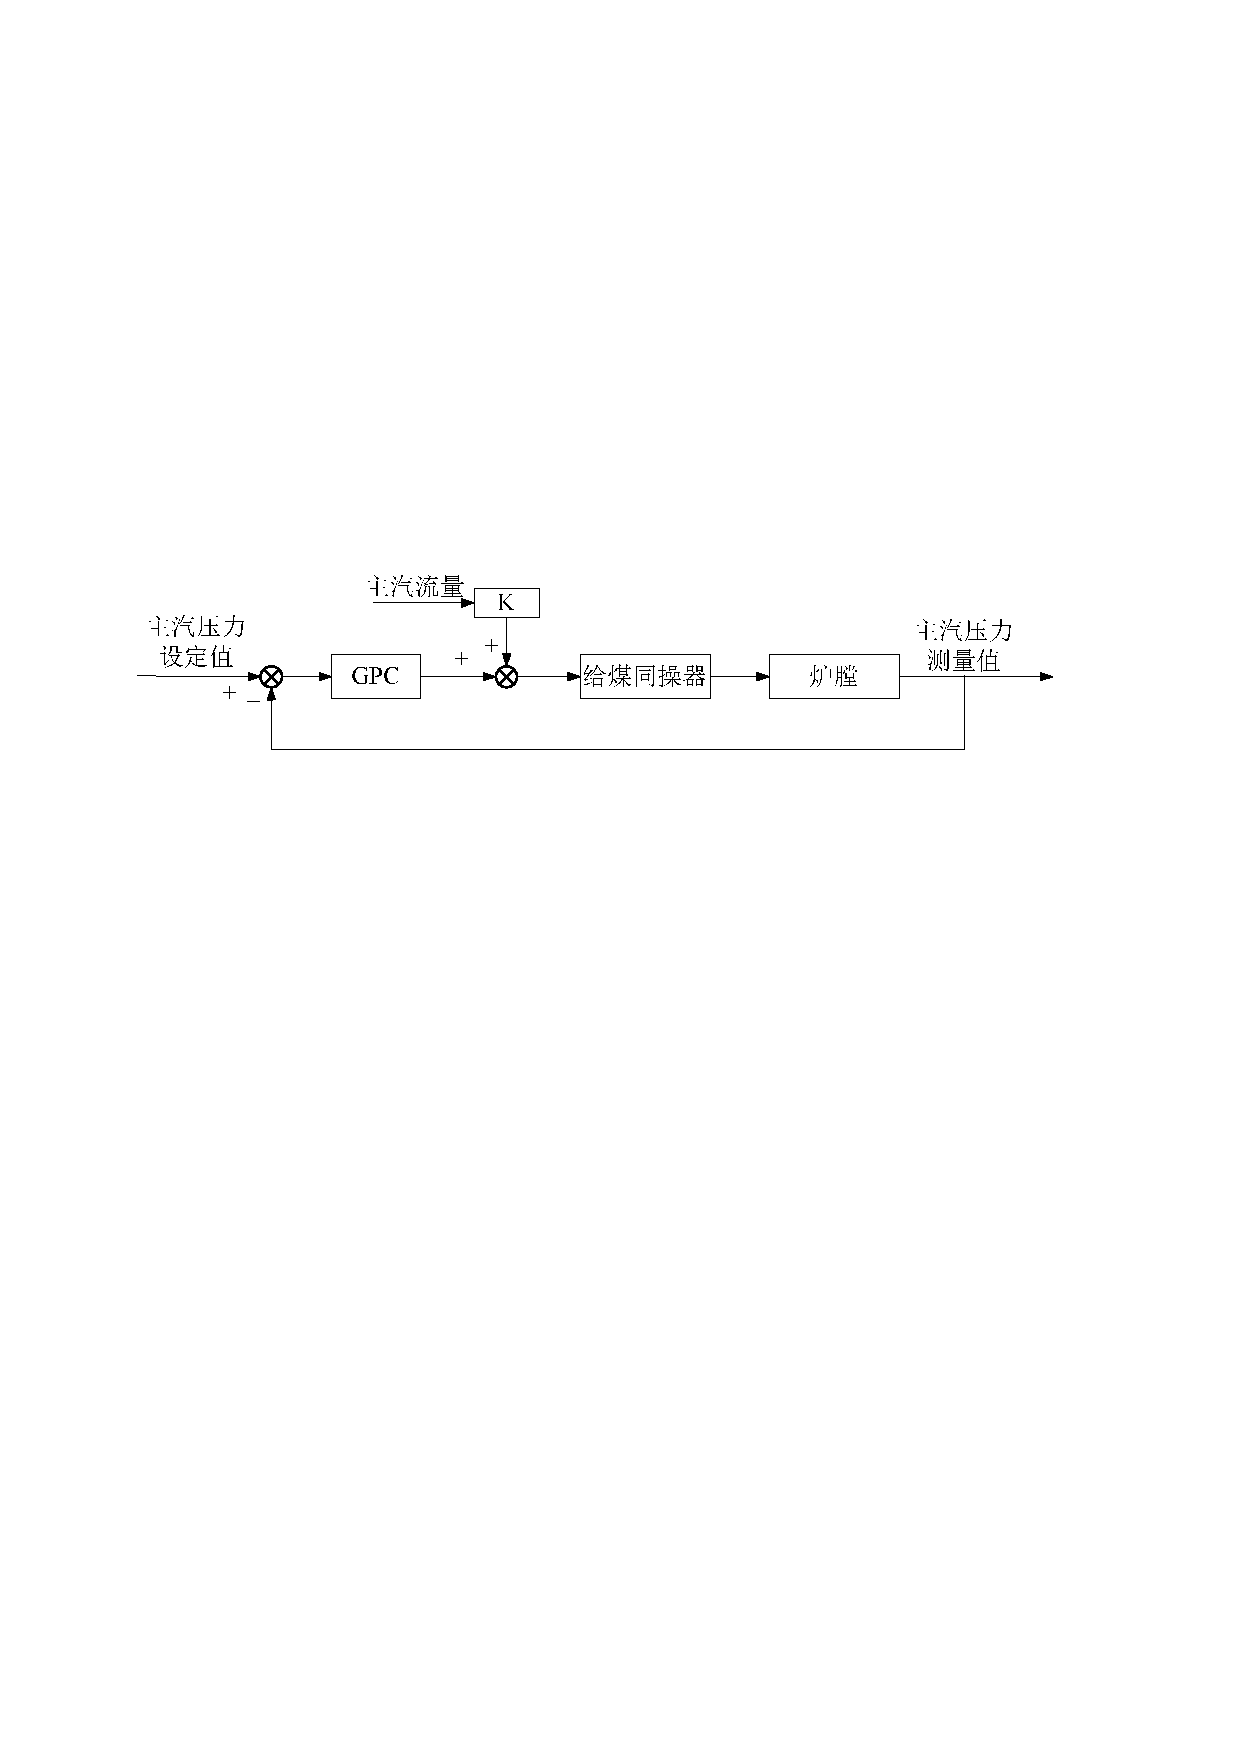
\includegraphics[width=13cm]{gas_pre_gpc}
\caption{主汽压力回路先进控制策略} \label{fig:gas_pre_gpc}
\end{figure}
\subsection{床温回路}
循环流化床锅炉中一次风量与给煤量都会影响床温。给煤量增大床温升高,一次风量增大,更多的热量被带到炉膛上部,床温降低。由于一次风的调节相对较快,且给煤量与一次风量之比会影响锅炉的流化状态。因此设计串级控制方案如图~\ref{fig:bed_tem_gpc}。使用一次风风煤比作为主回路控制输出,一次风风煤比与给煤量之积即为一次风量,通过双侧的一次风导叶开度来进行控制。
\begin{figure}[!hbt]
\centering
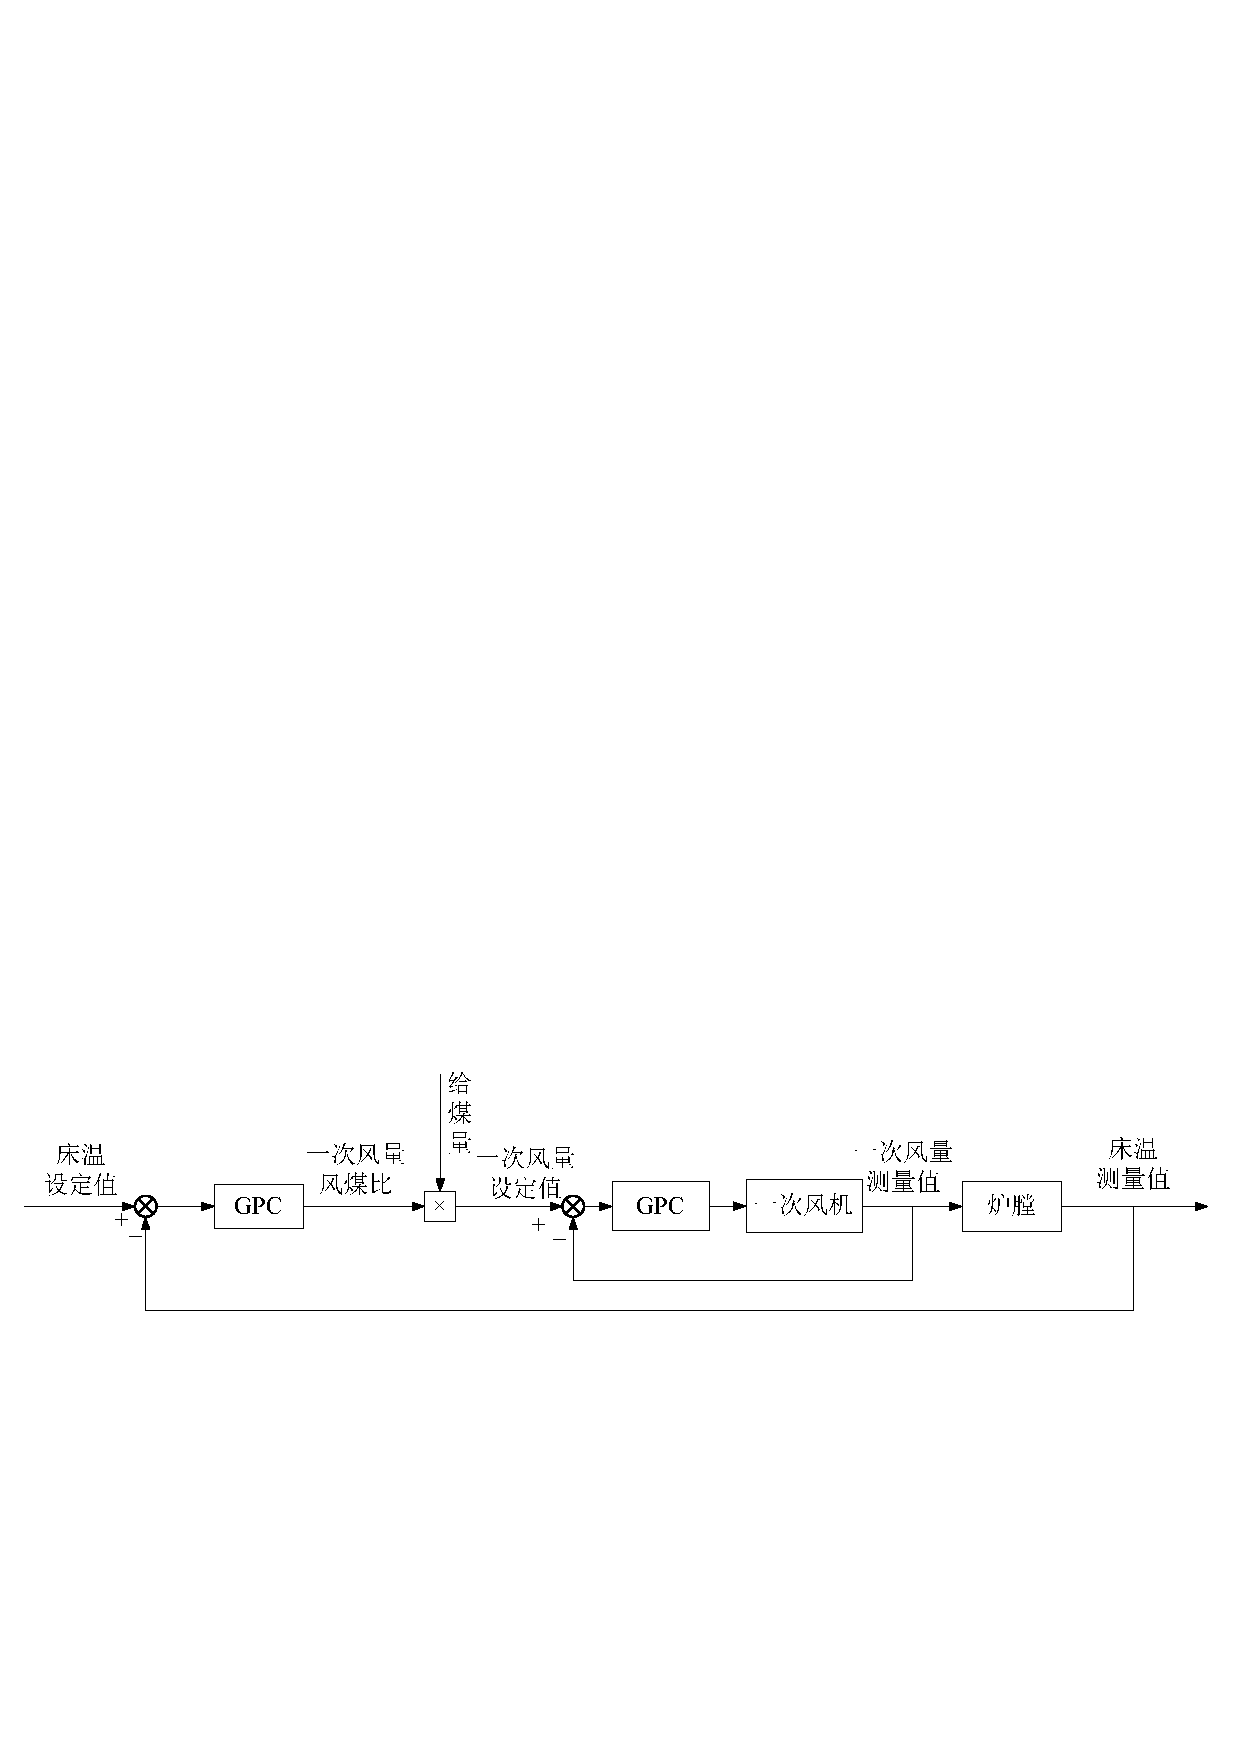
\includegraphics[width=14cm]{bed_tem_gpc}
\caption{床温回路先进控制策略} \label{fig:bed_tem_gpc}
\end{figure}
\begin{figure}[!hbt]
\centering
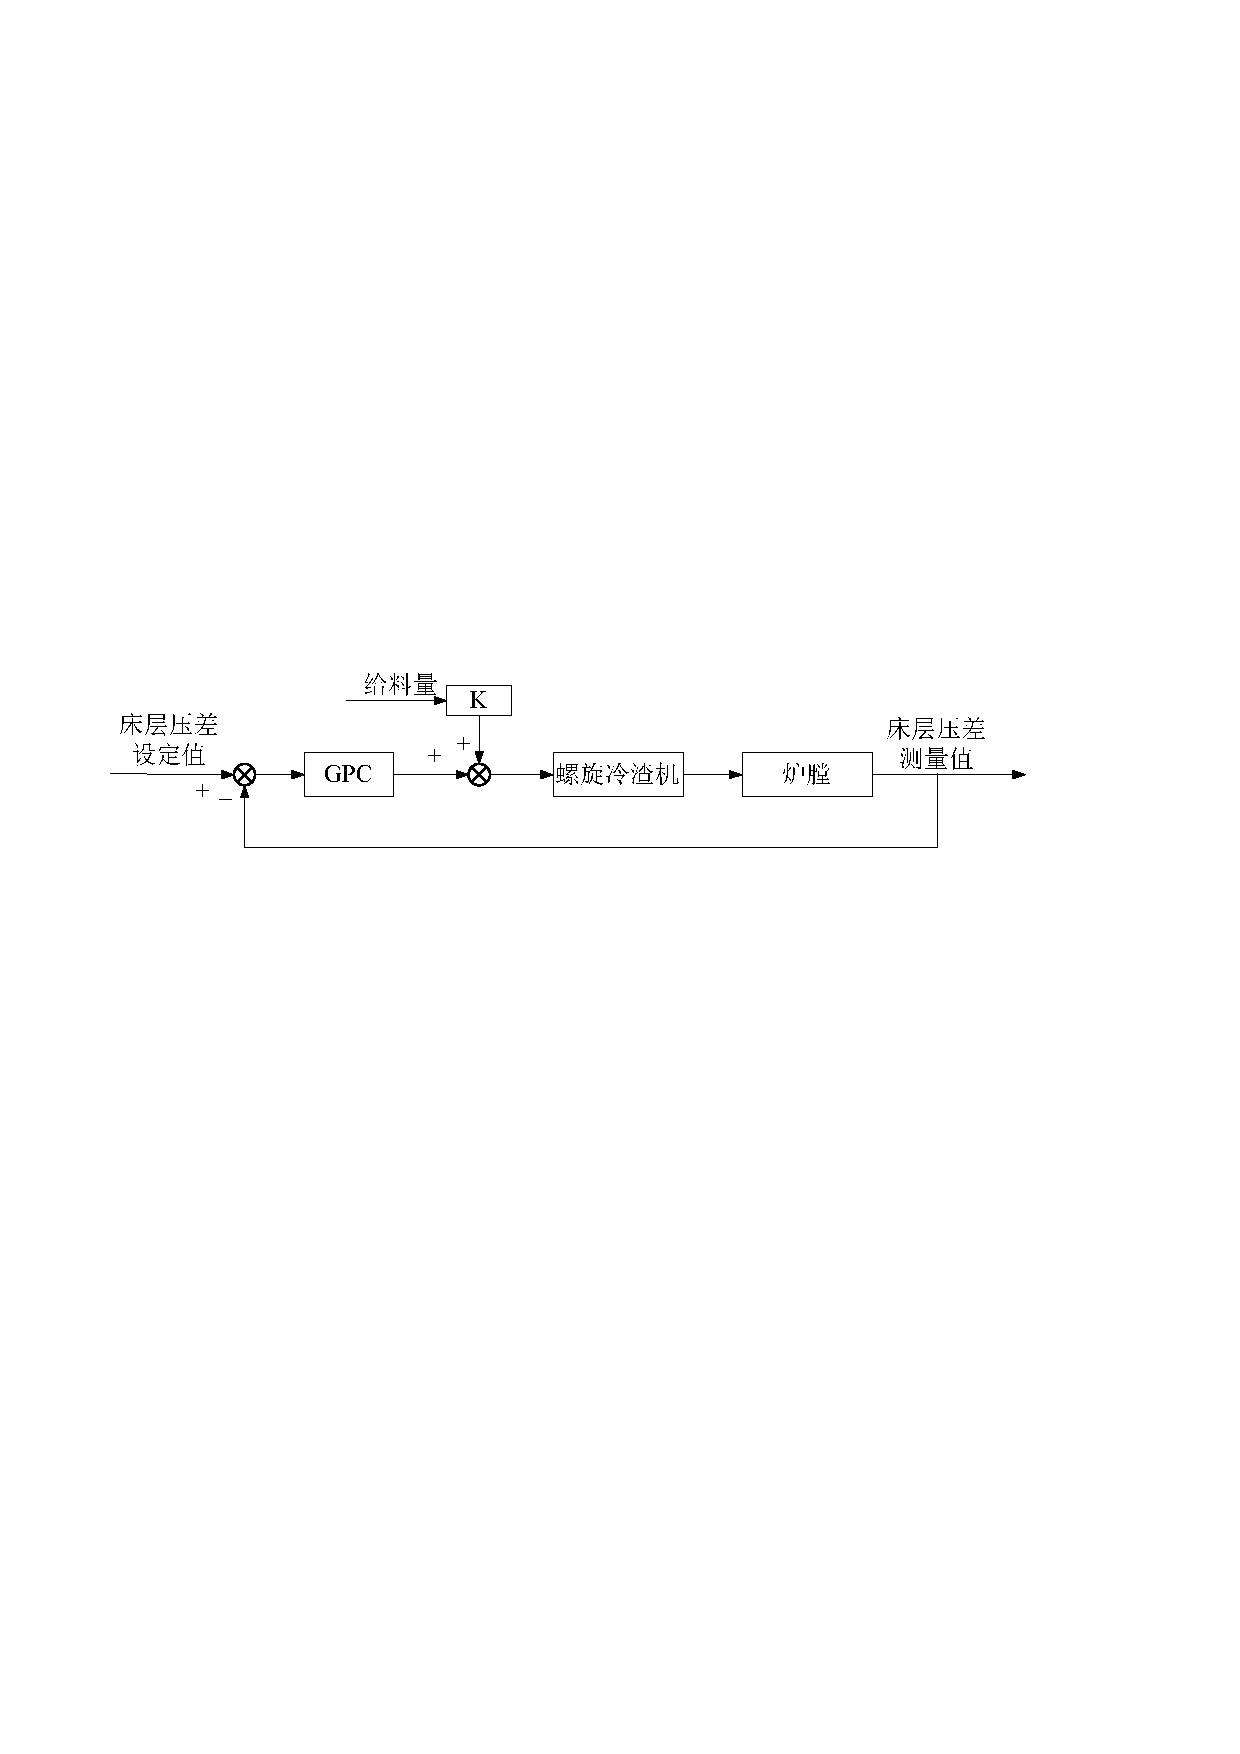
\includegraphics[width=13cm]{bed_pre_gpc}
\caption{床层压差回路先进控制策略} \label{fig:bed_pre_gpc}
\end{figure}
\subsection{床层压差回路}
床层压差回路主要受给料量和排渣量两个影响,这里的给料量是给煤量与石灰石量的总和。考虑到给煤量用来控制主汽压力,石灰石量用来调节~\ce{SO2},将排渣量作为控制床层压差的主要手段。采用单回路控制,如图~\ref{fig:bed_pre_gpc}~所示。通过螺旋冷渣机转速来调节床层压差,并增加针对给料量波动的前馈。




\section{先进控制系统设计及实现}
除了满足燃烧系统各回路控制目标外,先进控制系统还应尽量不破坏DCS系统原有的控制、告警、冷/热态启动、紧急停炉等功能。为了满足这一目标,先进控制系统运行在一台独立的工控机上,从DCS读取数据,完成控制量的计算后将控制量传输到DCS中,控制量的执行由DCS完成。
\subsection{硬件设计与实现}
硬件是先进控制软件运行的平台,为了尽可能避免先进控制系统对DCS的影响,采用如图~\ref{fig:adv_hardware}~所示的拓扑结构,实现先进控制与原有控制方式的的相对独立。先进控制软件在DCS之外的一台工控机上运行,通过OPC Server与DCS实现数据通讯。工控机采用ThinkServer机架式服务器,硬件配置按照现场需求随时更新,运行的操作系统为Windows Server 2008。
\begin{figure}[!hbt]
\centering
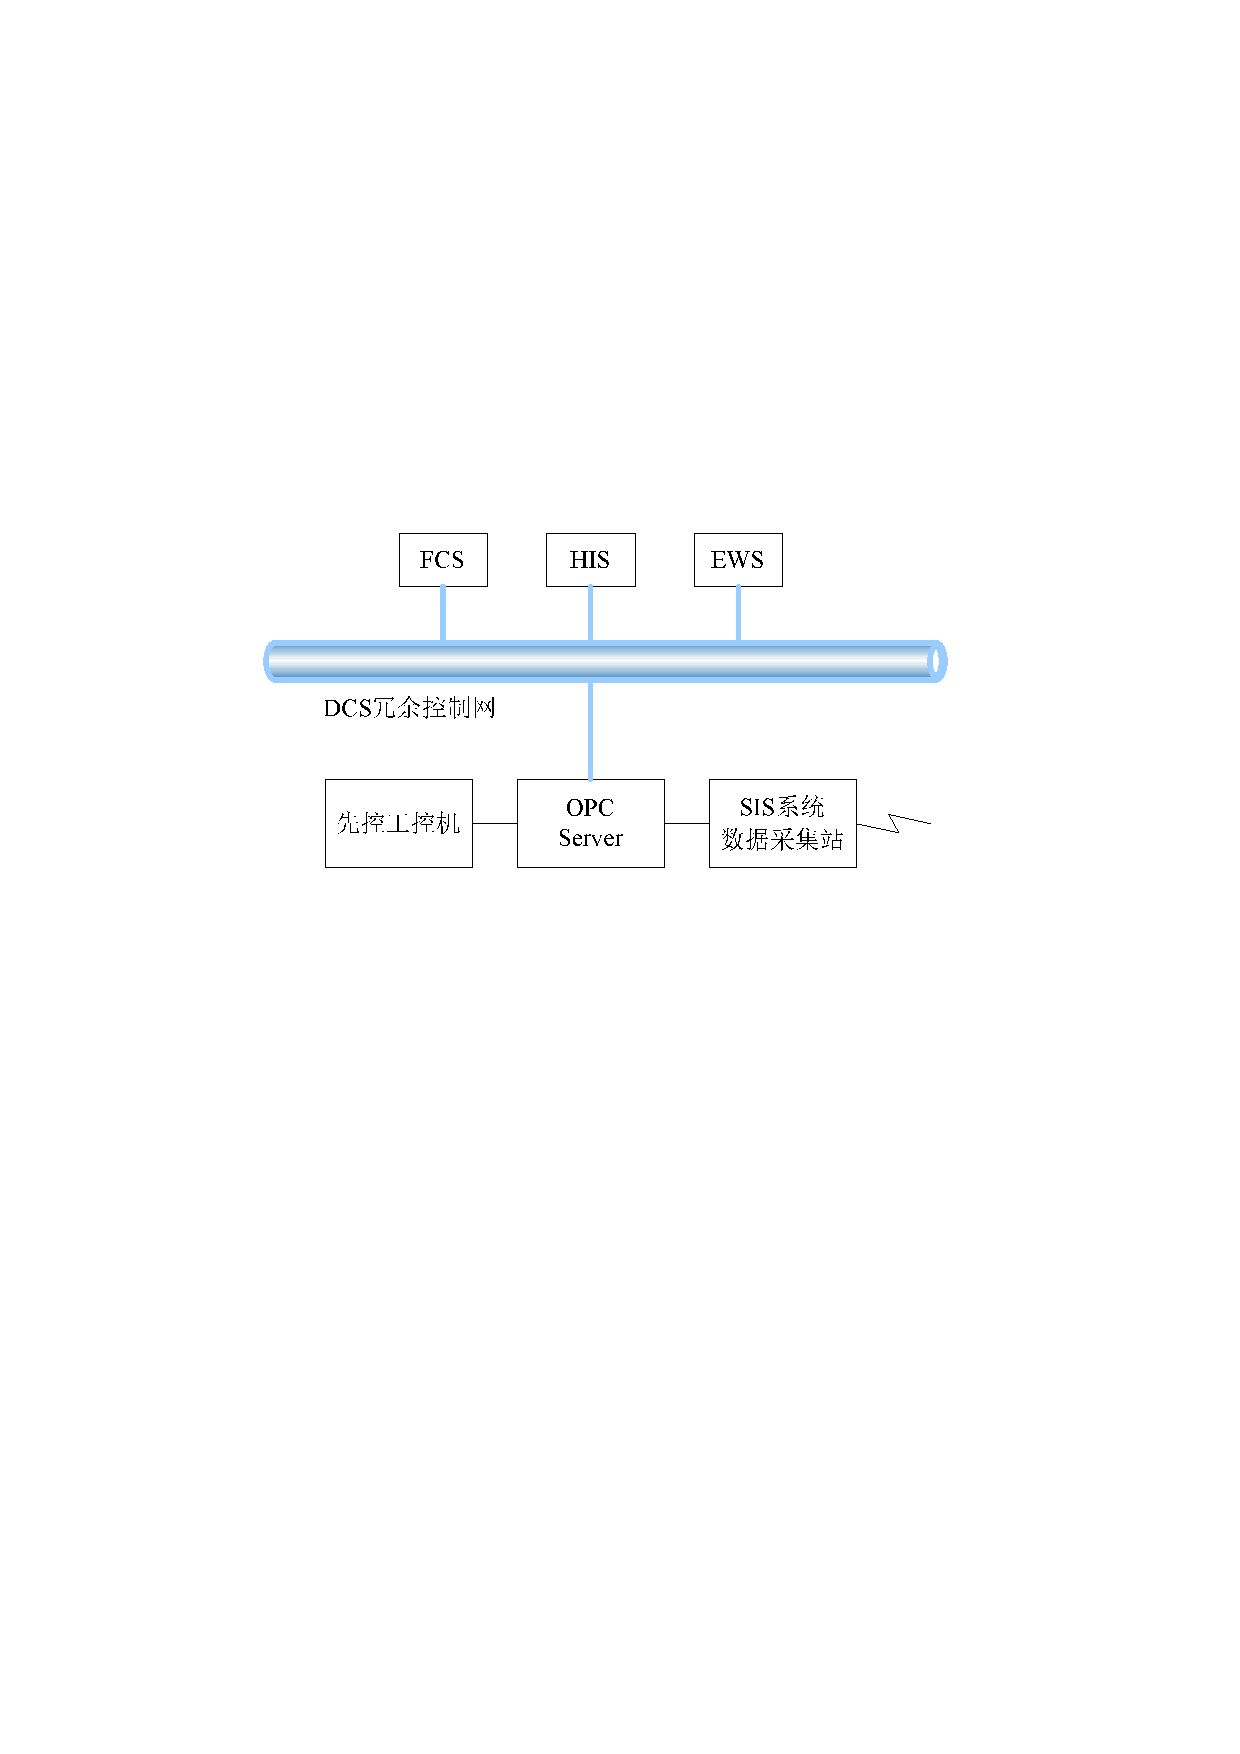
\includegraphics[width=9cm]{adv_hardware}
\caption{先进控制系统网络拓扑结构} \label{fig:adv_hardware}
\end{figure}
 
\subsection{软件设计与实现}
先进控制系统的软件部分是实现其功能的核心,主要由三大模块组成:数据通讯模块、实时趋势模块、控制算法模块。数据通讯模块完成先进控制软件与现场DCS系统的数据通讯,并将数据写入历史文件;实时趋势模块显示控制量和被控量实时曲线,便于工程师分析数据、整定控制器参数;控制算法模块利用数据通信模块的数据计算下一时刻的控制量,并将计算得出的控制量传回数据通讯模块。
\begin{figure}[!hbt]
\centering
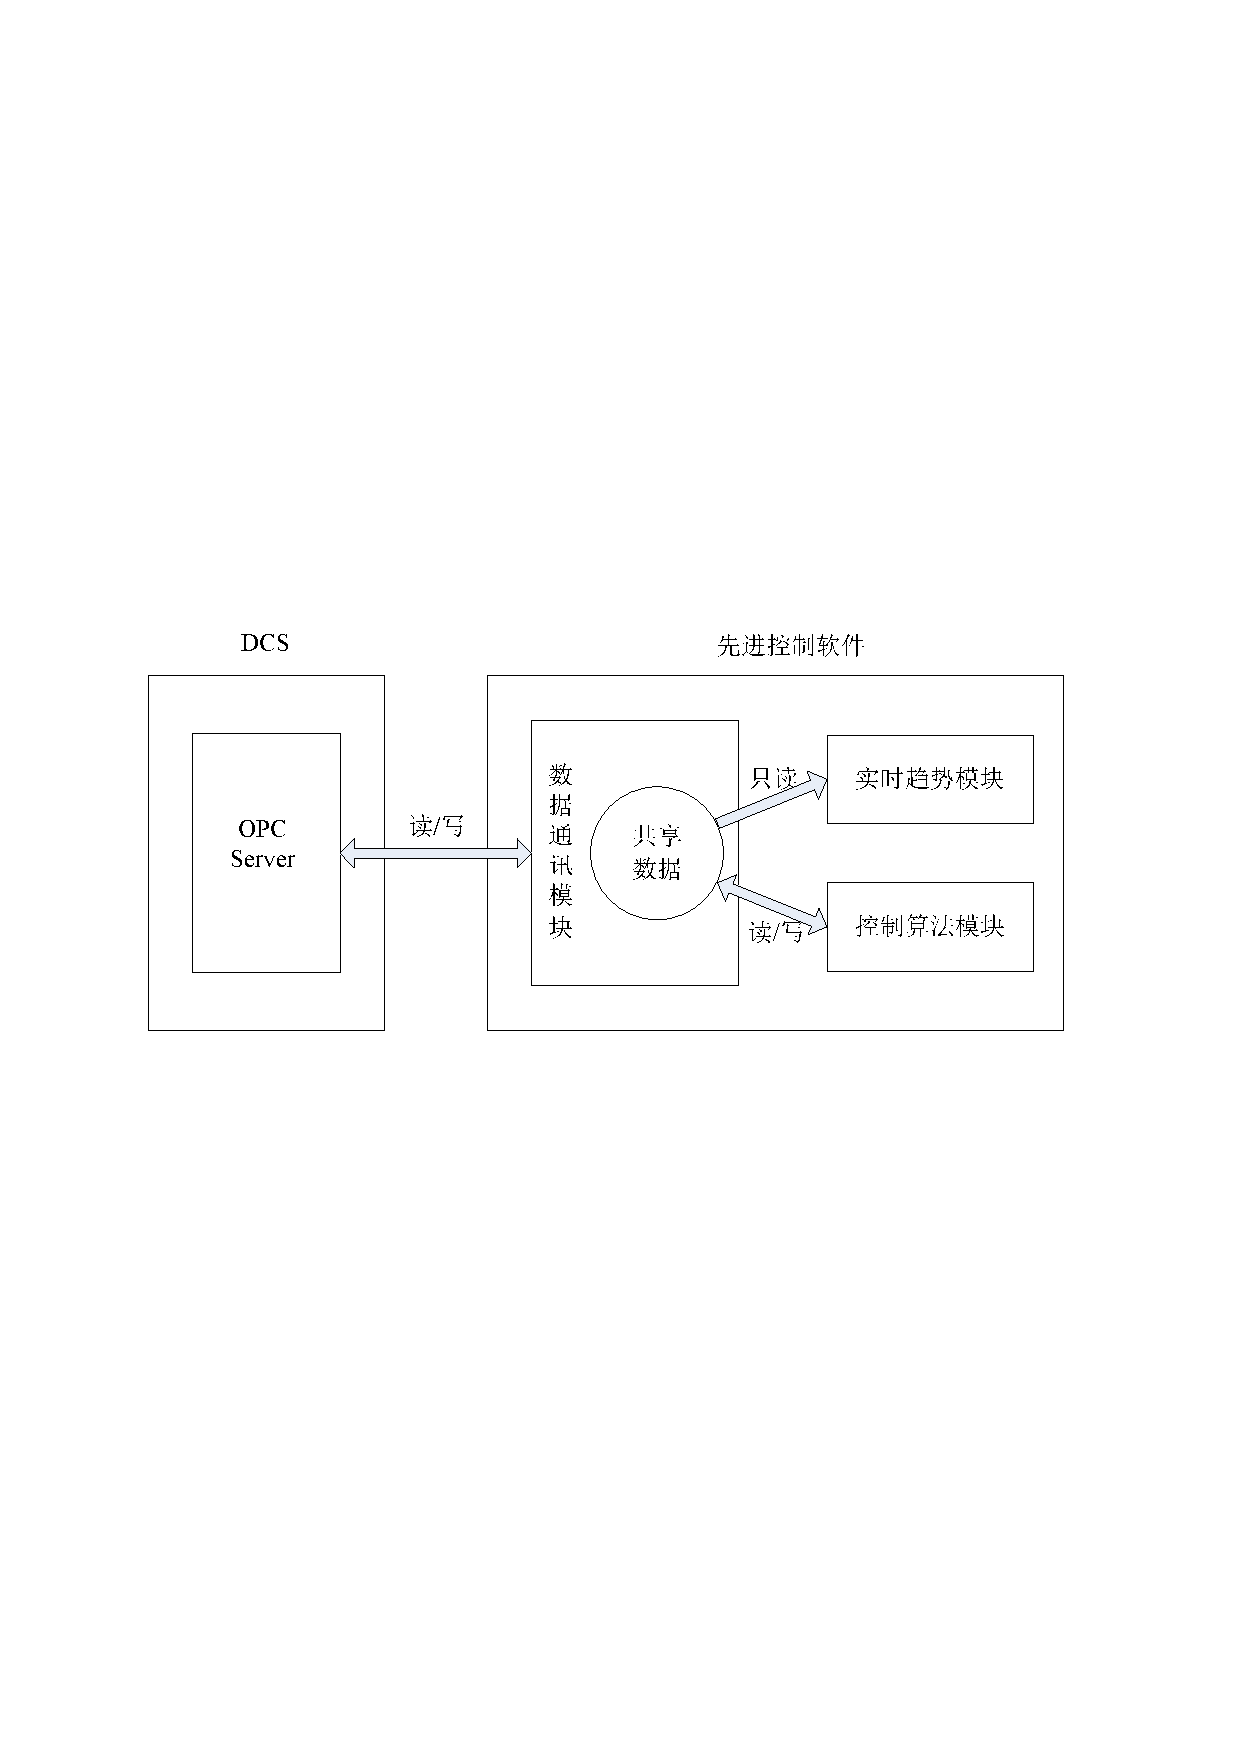
\includegraphics[width=10cm]{adv_software}
\caption{先进控制系统软件设计} \label{fig:adv_software}
\end{figure}

先控软件的开发采用Microsoft Visual C++ 6.0。数据通讯模块的开发基于Kepware Technologies的OPC Quick Client。在开源代码的基础上增加了将数据按天写入CSV(Comma-Separated Values,逗号分隔符)格式文件的功能。数据趋势模块基于RTD(Real-Time Data)技术,利用数据名在共享内存中查找相应数据并显示其实时趋势。先进控制模块实现广义预测控制算法,通过回路参数两个配置文件中的数据来对回路进行初始化,通过数据点参数读写相应变量。这样将控制算法和具体的回路分离,便于先进控制软件的复用和移植。

\section{先进控制系统投切逻辑设计及实现}
将软硬件部分配置完毕后,先进控制系统就能从DCS读取过程变量并将计算的控制量写回DCS。但为了让不同的控制量作用到相应的控制单元,且满足现场的控制要求,还需对DCS的组态进行一定的修改,实现数据通讯状态检测、投运开关、工艺条件不满足时自动切除先控、无扰切换等等。此外,先进控制系统应在DCS侧增加必要的监控画面、系统告警功能。


\subsection{数据传输监测}

只有当工控机与DCS数据传输状态良好时,先进控制系统与DCS正常交换数据。因此,必须有一定的机制保证先进控制投运时数据通讯正常。为此,可以设计随时间从0到100线性上升到100后归零的锯齿波信号(ALIVE信号),该信号由先进控制工控机内的先控软件输出至DCS系统,如图~\ref{fig:alive_signal}~所示。
\begin{figure}[!hbt]
\centering
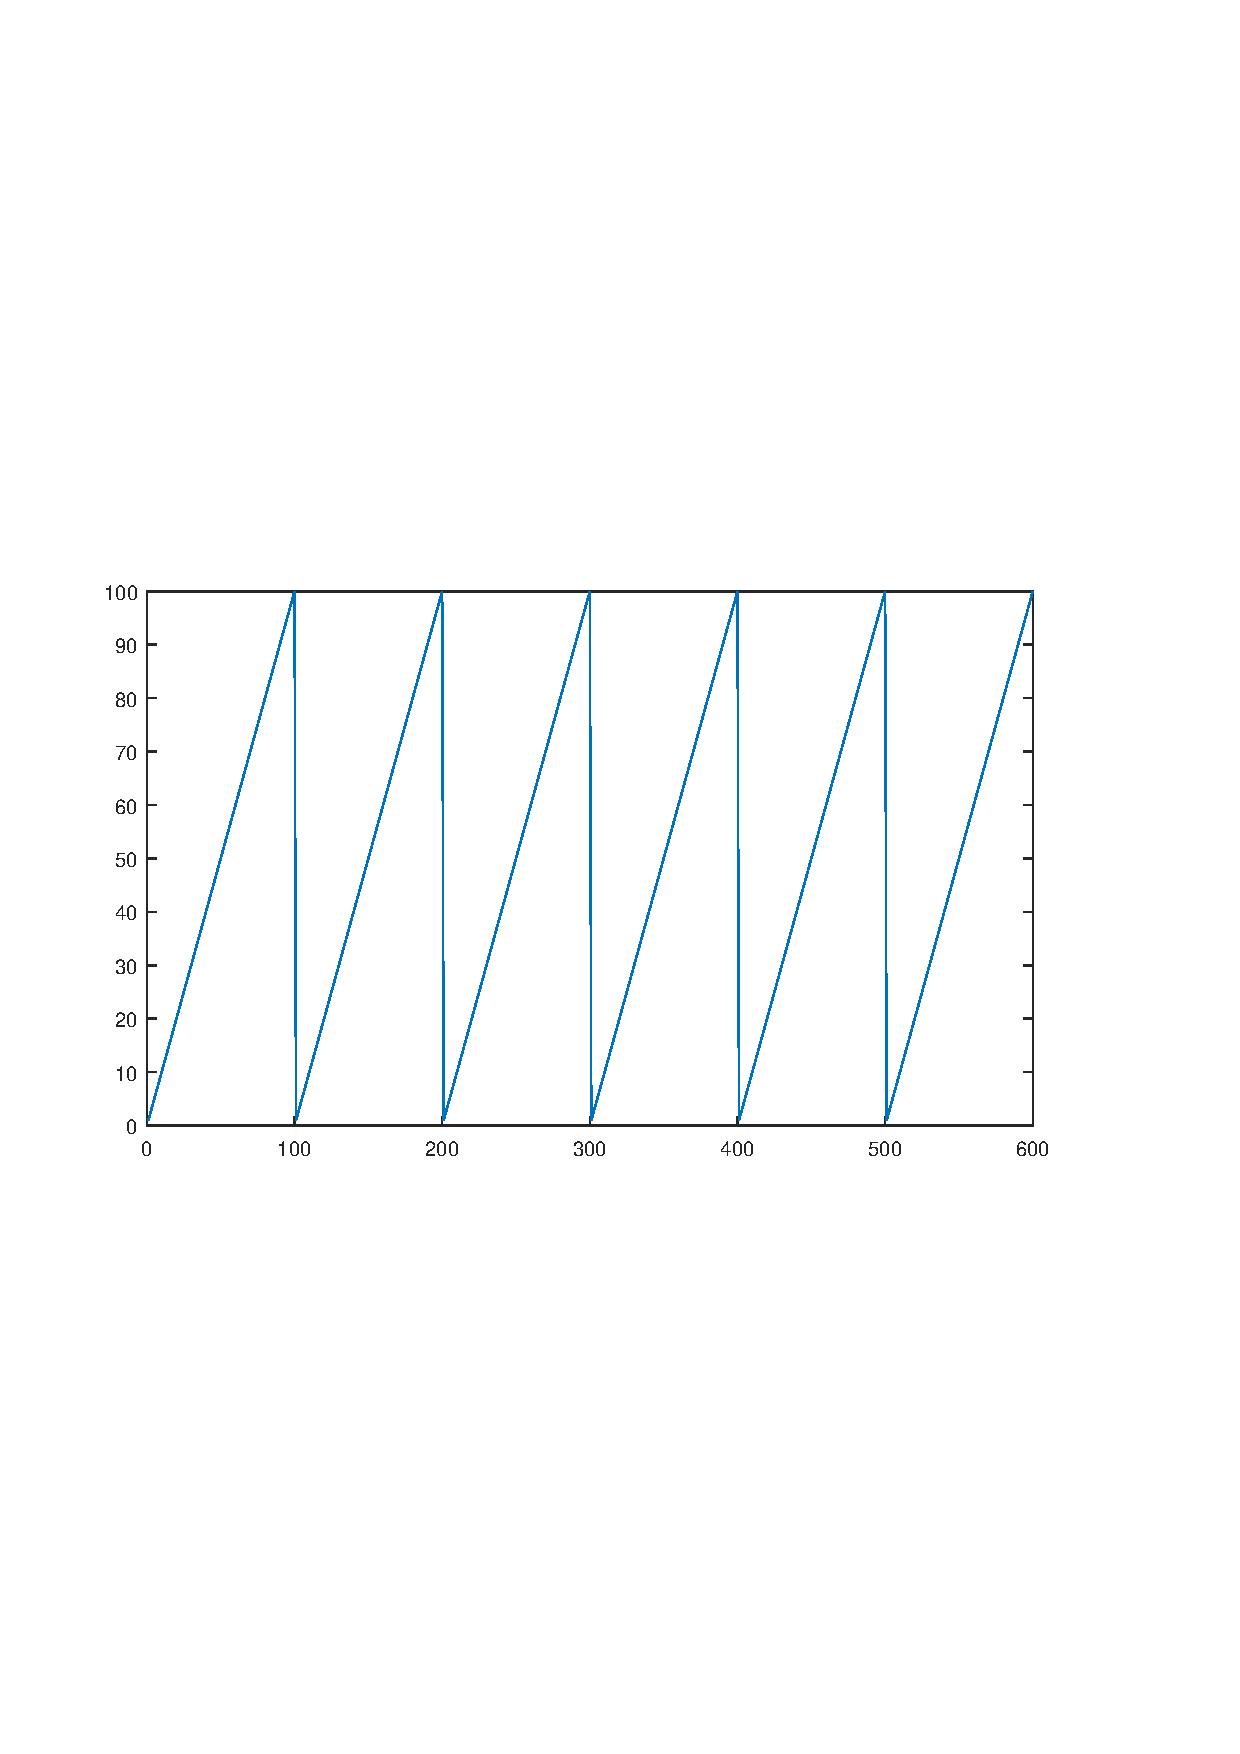
\includegraphics[width=12cm]{alive_signal}
\caption{先进控制系统生存信号} \label{fig:alive_signal}
\end{figure}

如果先进控制工控机与DCS系统之间出现通讯故障,在DCS系统的ALIVE信号将不再改变。在此基础上设计控制逻辑:如果ALIVE信号不再改变,将所有先控投运开关切换至手动,恢复至DCS系统手动控制。由于现场先进控制系统不仅仅包括燃烧系统,还包含汽包、减温水、风烟、空气预热器等系统。因此,ALIVE信号作用于整个先进控制系统,控制所有分系统的投运。
\begin{figure}[!hbt]
\centering
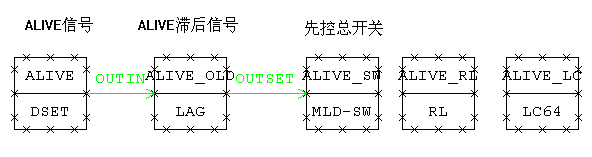
\includegraphics[width=12cm]{alive_logic}
\caption{先控总开关逻辑} \label{fig:alive_logic}
\end{figure}

系统内通过DSET模块接收ALIVE信号,通过LAG模块记录一步滞后的ALIVE信号,RL模块比较当前ALIVE信号和上一步ALIVE信号的大小关系。ALIVE$\_$SW为监测数据传输状态的开关,具有AUT(自动)和MAN(手动)两种模式。LC64模块利用RL模块的结果,当ALIVE信号与上一步ALIVE信号相等时,将先进控制总开关ALIVE$\_$SW置为手动状态;不等时,将其ALIVE$\_$SW置为AUT,如图~\ref{fig:alive_logic_eq}。
\begin{figure}[!hbt]
\centering
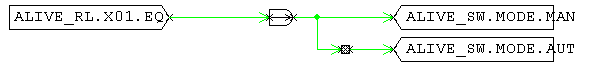
\includegraphics[width=12cm]{alive_logic_eq}
\caption{先控总开关切换逻辑} \label{fig:alive_logic_eq}
\end{figure}

 
图~\ref{fig:alive_logic_man}~为先控总开关为MAN模式下的逻辑。当先控开关为MAN时,将燃烧、风烟、减温水三个子系统的开关设置为MAN模式,并输出一个报警信号,通知操作人员先控已被切除。
\begin{figure}[!hbt]
\centering
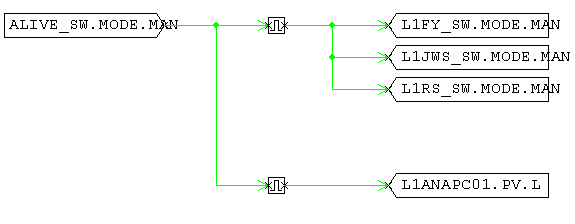
\includegraphics[width=13cm]{alive_logic_man}
\caption{先控总开关控制逻辑} \label{fig:alive_logic_man}
\end{figure}

 
\subsection{燃烧子系统投切逻辑}
先进系统的投切开关分为三类:先控总开关、子系统开关和回路开关。三者共同协作,保证先控投切顺利进行。这些开关都通过MLD-SW模块实现。除了先控总开关,其它开关都提供了供操作人员操作的按钮。子系统开关可供操作人员操作,控制子系统内的所有回路。这个开关作为先控总开关与回路开关的桥梁,既不监测先控生存信号,也不监测系统当前的工艺条件。当子系统开关置为MAN时,子系统内所有回路开关自动切换到MAN状态。只有子系统开关为AUT时,回路开关才允许置为AUT。表~\ref{tab:burnning_state}~给出了燃烧子系统中可能的开关状态,AUT/MAN表示允许AUT和MAN两种状态。

\begingroup
\renewcommand*{\arraystretch}{1.67}
\begin{table}[!h]
\small
\centering
\caption[燃烧子系统状态]{燃烧子系统状态} \label{tab:burnning_state}
\begin{tabular}{cccc}
\hline\hline
燃烧系统开关&主汽压力回路开关&床温回路开关&床层压差回路开关\\
MAN&MAN&MAN&MAN\\
AUT&AUT/MAN&AUT/MAN&AUT/MAN\\
\hline\hline
\end{tabular}
\end{table}
\endgroup

\begin{figure}[!hbt]
\centering
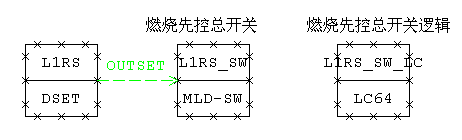
\includegraphics[width=10cm]{burn_logic}
\caption{燃烧子系统逻辑} \label{fig:burn_logic}
\end{figure}
 
图~\ref{fig:burn_logic}~为DCS系统中燃烧子系统开关的逻辑,其实现方式与先控总开关类似。采用MLD-SW模块作为开关,LC64模块控制回路开关状态,并输出先进控制投切报警信号。

\subsection{主汽压力回路投切逻辑}
回路也有操作按钮,仅控制单回路的投切。为了保障先控系统的运行安全,回路需要满足一定的工艺条件后才能投运。投运后,先进控制系统计算出的控制量也需要通过回路开关内部的逻辑作用到执行机构。下面以主汽压力回路为例,阐述回路投切的逻辑。

\begin{figure}[!hbt]
\centering
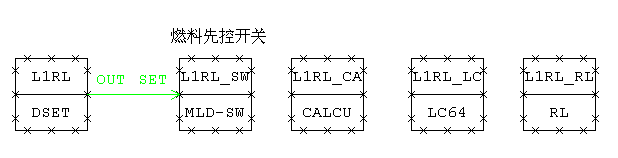
\includegraphics[width=13cm]{coal_logic}
\caption{主汽压力回路燃料量逻辑} \label{fig:coal_logic}
\end{figure}
 
图~\ref{fig:coal_logic}~为DCS系统内燃料量的逻辑图。利用DSET模块接收先进控制系统计算出的物理量,MLD-SW 模块判断当前回路的状态,RL比较工艺条件,LC64实现具体的回路投切逻辑。
先进控制系统必须在工况较为稳定的条件下才能投运。因此,需要设计一系列工艺范围,当要求的变量在制定范围内,才允许投运先控。工艺范围外即为先进控制切除条件,系统满足任意一个切除条件就要立刻切除,如图~\ref{fig:switch_logic}~所示。

\begin{figure}[!hbt]
\centering
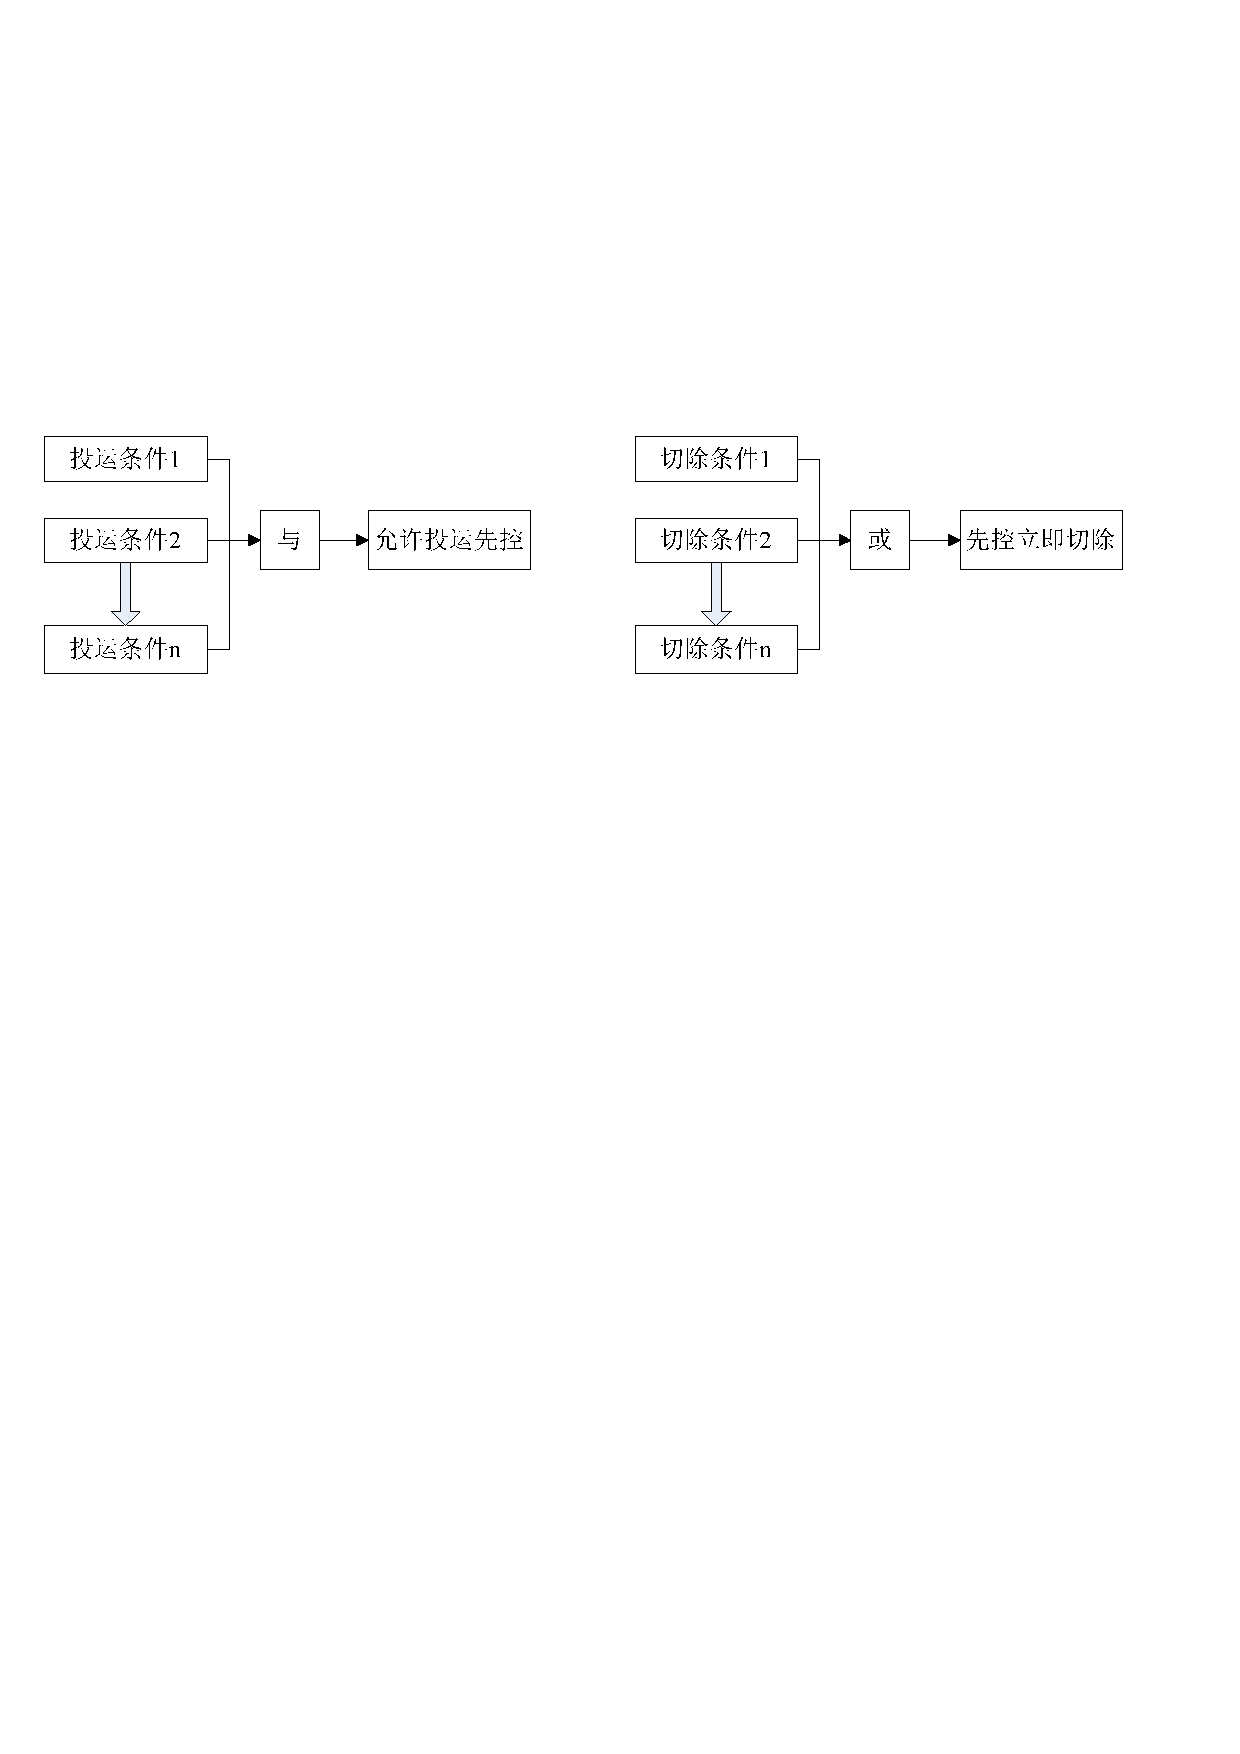
\includegraphics[width=11cm]{switch_logic}
\caption{回路投切逻辑} \label{fig:switch_logic}
\end{figure}

在实际系统中,受各种环境、组分等因素影响,经常有不确定的扰动作用于控制系统。如果先控系统在变量超出工艺范围时就立即切除,在进入工艺要求范围内就立即投运,这样会导致系统频繁切换控制方式,影响先进控制的效果。因此,现场设计的投切条件不仅要求变量处于一定的区间范围,还要求变量在这段区间内保持一定的时间,之后进行先控的投切。

\begin{figure}[!hbt]
\centering
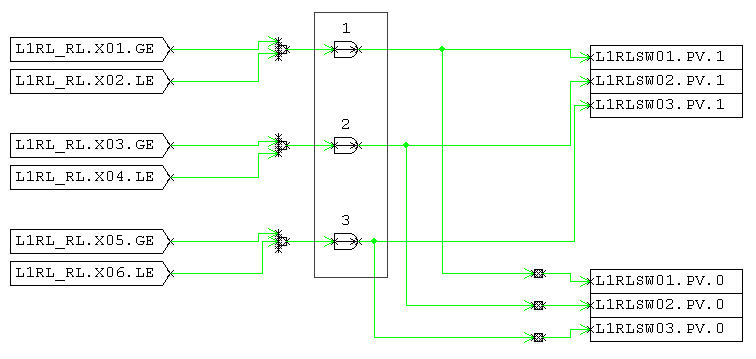
\includegraphics[width=13cm]{coal_logic_delay}
\caption{主汽压力回路延时逻辑} \label{fig:coal_logic_delay}
\end{figure}
 
利用DCS提供的OND模块提供的上升沿延时功能,可以实现先进控制投切的延时处理。图~\ref{fig:coal_logic_delay}~为主汽压力回路的一部分逻辑。当变量满足要求时,OND的输入量变为1,经过预先设定的时间后,其输出量才变为1。这时,控制回路先控开关的信号才为1。

\begin{figure}[!hbt]
\centering
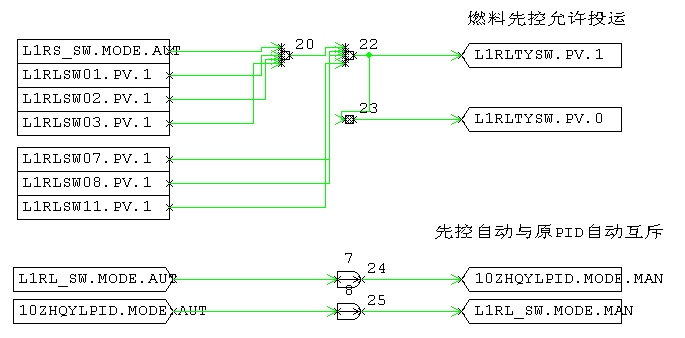
\includegraphics[width=13cm]{coal_logic_aut}
\caption{主汽压力回路投切逻辑} \label{fig:coal_logic_aut}
\end{figure}

图~\ref{fig:coal_logic_aut}~为主汽压力回路的另一部分逻辑。通过与运算保证直到所有控制回路开关的信号都为1,才允许该回路投运先进控制。这里可以看到,该回路投运先进控制的前提条件是燃烧系统开关为AUT状态。另外,附加了保证先进控制与原有PID自动控制互斥的逻辑。回路投切也有相应的报警信号,与先控总开关中的实现类似。
  
\subsection{回路无扰切换}

\begin{figure}[!hbt]
\centering
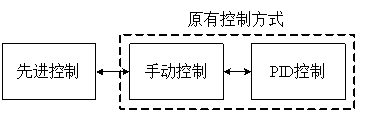
\includegraphics[width=9cm]{bumpless_logic}
\caption{无扰切换逻辑} \label{fig:bumpless_logic}
\end{figure}
 
无扰切换保证控制方式改变时控制量不会发生突变,从而提高系统的稳定性和执行机构的寿命。在先进控制系统投运之前,现场已有手动控制和PID自动控制两种控制方式。PID控制与先进控制系统类似,都只能在系统工况比较稳定的状态下运行。当操作人员切除先进控制的时候,现场工况一般也不能满足PID控制的要求。因此,将手动控制作为系统无扰切换的中间状态,系统的投切路径如图~\ref{fig:bumpless_logic}~所示。先进控制系统只有在系统为手动控制的时候才能投运,先进控制切除时系统自动切回手动控制状态。

当先进控制投运时,先进控制系统计算的控制信号直接传送给手操器,执行机构接着执行相应动作。当切除先进控制时,手操器信号作用于执行机构,先控的控制量应当跟踪手操器的输出值。这样,系统中不同的控制方式的控制量始终保持一致,控制方式的切换不会引起状态突变。

\begin{figure}[!hbt]
\centering
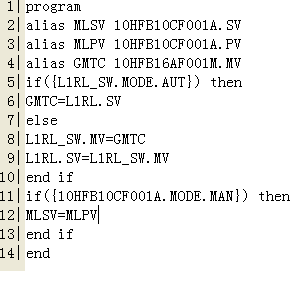
\includegraphics[height = 5cm]{bumpless_pro}
\caption{无扰切换程序} \label{fig:bumpless_pro}
\end{figure}

仍以主汽压力回路为例。除了保障回路安全投切的逻辑外,在CALCU模块中还有利用SEBOL语言来实现无扰切换的程序。除了实现无扰切换外,还设定手动控制状态时将过程测量值赋给设定值,保证系统输出与设定值一致。
 
\subsection{回路投切条件汇总}
\label{sec:loop_req}

燃烧系统涉及的所有回路都必须在燃烧系统开关为AUT状态时才能投运先进控制。主汽压力回路的投切条件如表~\ref{tab:gas_pre_req}~所示。另外,由于床温和氧量对系统燃烧状态影响较大,主汽压力回路应在床温—一次风回路和氧量—二次风回路投运先进控制之后投运。

\begingroup
\renewcommand*{\arraystretch}{1.67}
\begin{table}[!h]
\small
\centering
\caption[主汽压力先进控制投切工艺条件]{主汽压力先进控制投切工艺条件} \label{tab:gas_pre_req}
\begin{tabular}{cccc}
\hline\hline
变量	&投运条件&	切除条件&	许可范围\\
\hline
主汽压力变化量&范围内保持60$\,$\si{s}&	范围外保持30$\,$\si{s}&	$[\textrm{-0.1},\,\textrm{0.1}]\,$\si{\mega\pascal}\\
主汽压力	&范围内保持60$\,$\si{s}	&范围外保持30$\,$\si{s}	&$[\textrm{9.3},\,\textrm{9.7}]\,$\si{\mega\pascal}\\
给煤同操器	&范围内保持60$\,$\si{s}	&范围外保持30$\,$\si{s}	&$[\textrm{6.5},\,\textrm{8}]\,$\si[per-mode=symbol]{\tonne\per\hour}\\
床温	&范围内保持60$\,$\si{s}	&范围外保持30$\,$\si{s}&	$[\textrm{900},\,\textrm{930}]\,$\si{\degreeCelsius}\\
给煤量	&范围内保持60$\,$\si{s}	&范围外保持30$\,$\si{s}	&$[\textrm{40},\,\textrm{50}]\,$\si[per-mode=symbol]{\tonne\per\hour}\\
\hline\hline
\end{tabular}
\end{table}
\endgroup


床温回路的先控投切工艺条件如表~\ref{tab:bed_tem_req}~所示,由于床温回路采用串级控制策略,其主回路输出风煤比,副回路控制一次风。因此,床温回路需要在一次风回路稳定运行后才能投运自动。表~\ref{tab:flow_req}~为一次风先进控制投切条件。

\begingroup
\renewcommand*{\arraystretch}{1.67}
\begin{table}[!h]
\small
\centering
\caption[床温先进控制投切工艺条件]{床温先进控制投切工艺条件} \label{tab:bed_tem_req}
\begin{tabular}{cccc}
\hline\hline
变量	&投运条件	&切除条件	&许可范围\\
\hline
床温变化量	&范围内保持60$\,$\si{s}	&范围外保持30$\,$\si{s}	&$[\textrm{-10},\,\textrm{10}]\,$\si{\degreeCelsius}\\
床温	&范围内保持60$\,$\si{s}	&范围外保持30$\,$\si{s}	&$[\textrm{900},\,\textrm{930}]\,$\si{\degreeCelsius}\\
风煤比反馈	&范围内保持60$\,$\si{s}	&范围外保持30$\,$\si{s}	&$[\textrm{2.2},\,\textrm{3.3}]$\\
床层压力	&范围内保持60$\,$\si{s}	&范围外保持30$\,$\si{s}&	$[\textrm{7.5},\,\textrm{9}]\,$\si{\kilo\pascal}\\
\hline\hline
\end{tabular}
\end{table}
\endgroup


\begingroup
\renewcommand*{\arraystretch}{1.67}
\begin{table}[!h]
\small
\centering
\caption[一次风先进控制投切条件]{一次风先进控制投切条件} \label{tab:flow_req}
\begin{tabular}{cccc}
\hline\hline
变量	&投运条件	&切除条件	&许可范围\\
\hline
一次风量变化量	&范围内保持60$\,$\si{s}	&范围外保持30$\,$\si{s}	&$[\textrm{-30},\,\textrm{30}]\,$\si[per-mode=symbol]{\kilo\meter^{3}\per\hour}\\
一次风量	&范围内保持60$\,$\si{s}	&范围外保持30$\,$\si{s}	&$[\textrm{105},\,\textrm{170}]\,$\si[per-mode=symbol]{\kilo\meter^{3}\per\hour}\\
一次风机入口导叶开度	&范围内保持60$\,$\si{s}	&范围外保持30$\,$\si{s}	&$[\textrm{10},\,\textrm{50}]\,$\si{\percent}\\
\hline\hline
\end{tabular}
\end{table}
\endgroup


床层压差回路的先控投切条件如表~\ref{tab:bed_pre_req}。该回路仅对炉内留存的床料量由影响,在实际中最先投运。

\begingroup
\renewcommand*{\arraystretch}{1.67}
\begin{table}[!h]
\small
\centering
\caption[床层压差先控投切条件]{床层压差先控投切条件} \label{tab:bed_pre_req}
\begin{tabular}{cccc}
\hline\hline
变量	&投运条件	&切除条件	&许可范围\\
\hline
床层压差变化量	&范围内保持60$\,$\si{s}&	范围外保持30$\,$\si{s}&	$[\textrm{-1},\,\textrm{1}]\,$\si{\kilo\pascal}\\
床层压差	&范围内保持60$\,$\si{s}	&范围外保持30$\,$\si{s}	&$[\textrm{5.5},\,\textrm{8}]\,$\si{\kilo\pascal}\\
冷渣机转速	&范围内保持60$\,$\si{s}	&范围外保持30$\,$\si{s}	&$[\textrm{150},\,\textrm{400}]\,$\si{r/\min}\\
\hline\hline
\end{tabular}
\end{table}
\endgroup

所有的投运条件都需要让变量在范围内保持60$\,$\si{s},而切除条件只需变量在范围外保持30$\,$\si{s}。这样保证了先进控制系统只能在系统较稳定时候投运,在工况不稳定的时候及早切除,提高了现场的安全性。

\begin{figure}[!hbt]
\centering
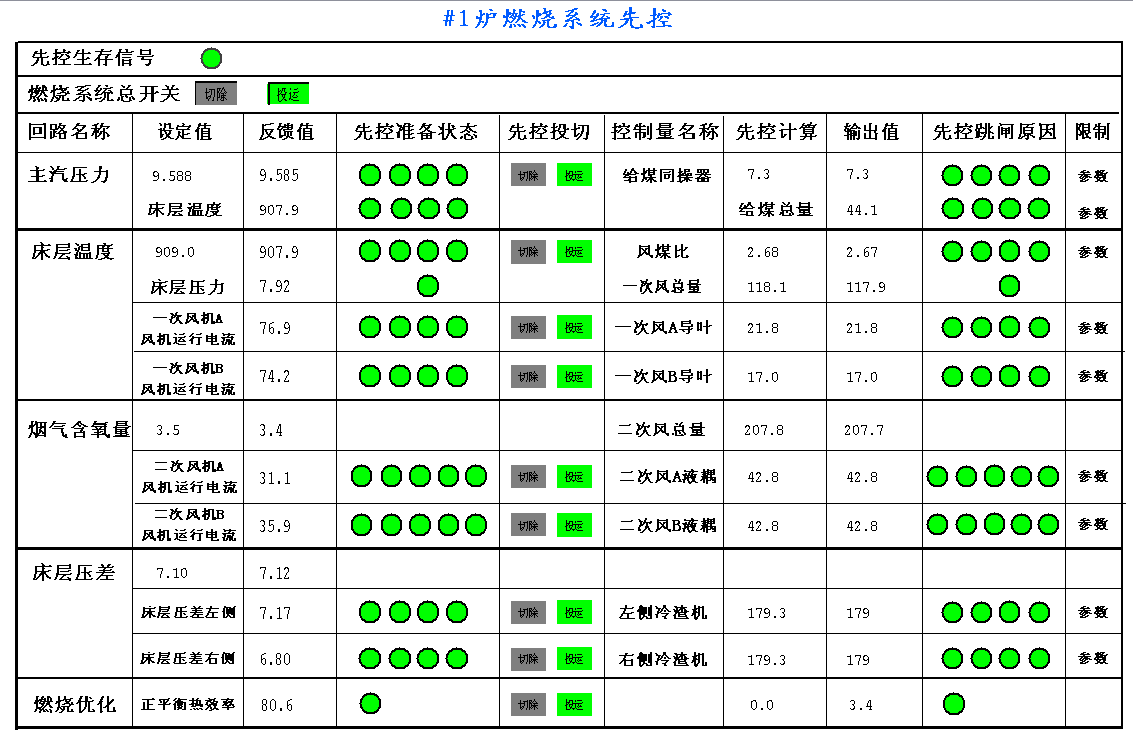
\includegraphics[width = 13cm]{adv_con_his}
\caption{先控投运画面} \label{fig:adv_con_his}
\end{figure}

\begin{figure}[!hbt]
\centering
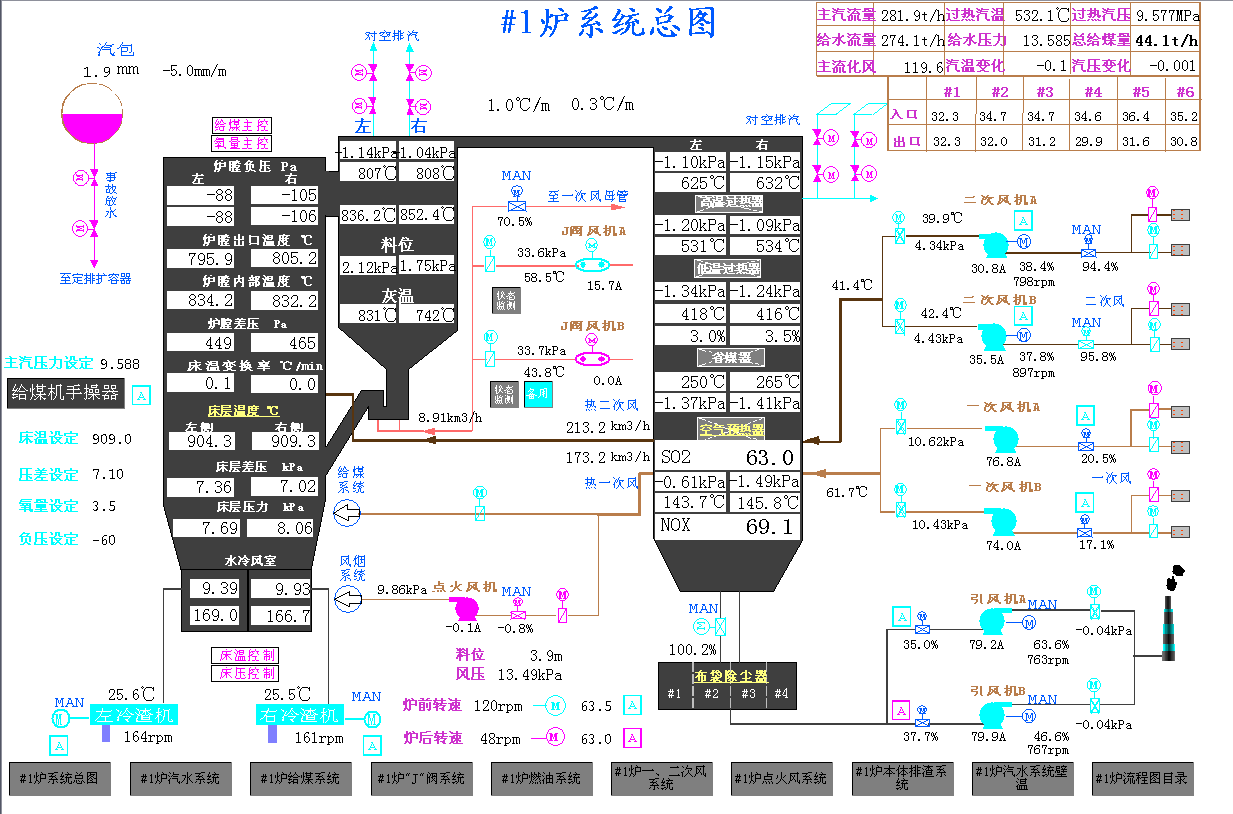
\includegraphics[width = 13cm]{final_his}
\caption{锅炉监控画面} \label{fig:final_his}
\end{figure}

\section{先进控制监控画面设计与实现}  

在完成投切逻辑后,还应设计并实现先进控制的监控画面,这样操作人员才能方便地在HIS站对先进控制系统进行操作,如图~\ref{fig:adv_con_his}~。先控准备状态的设置如~\ref{sec:loop_req}~节所述。当满足条件时,其颜色变为绿色,否则变为红色。点击图中的圆点,提示了该圆点的内容和现在的状态。点击最后一列的“参数”,则显示该回路的限制参数。这些参数在操作员站没有修改权限,只能在工程师站进行修改。


除此之外,在系统总图的相关区域,增加先控的设定值显示、先控投用切除状态显示和快捷切除按钮,如图~\ref{fig:final_his}。在流程图目录中增加先进控制的相关目录。

\section{本章小结}
本章首先介绍了广义预测控制算法,并基于广义预测控制器设计了燃烧系统各回路的控制策略。随后介绍了先进控制系统的软硬件设计和实现,保证了先进控制系统与原有系统的相对独立。为了让操作人员能够在控制室集中操作、监控先进控制系统,利用CS 3000提供的工程技术功能对DCS侧的组态做一定的修改和添加,包括先进控制系统生存信号、燃烧系统投切总开关、各回路投切条件和逻辑、监控画面等。